\documentclass{standalone}
\usepackage{tikz}
\usepackage{ctex,siunitx}
\usepackage{tkz-euclide}
\usepackage{amsmath}
\usetikzlibrary{patterns,calc}
\usetikzlibrary {decorations.pathmorphing, decorations.pathreplacing, decorations.shapes}
\begin{document}
\small
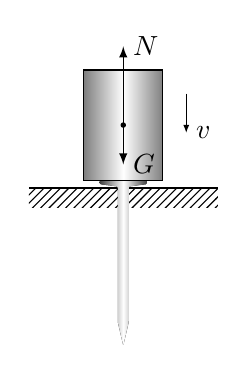
\begin{tikzpicture}[>=latex, scale=1]
  \fill[pattern=north east lines](-1.2,-0.25)rectangle(1.2,0);
  \draw[thick](-1.2,0)--(1.2,0);
  \fill[left color=darkgray,right color=darkgray, middle color=white,rounded corners=0.15mm](-0.3,0.1)--(0.3,0.1)--(0.3,0.05)--(0.07,0.02)--(0.07,-1.7)--(0,-2.0)--(-0.07,-1.7)--(-0.07,0.02)--(-0.3,0.05)--cycle;
  \fill[draw=black,left color=gray,right color=gray, middle color=white](-0.5,0.1)rectangle(0.5,1.5);
  \fill(0,0.8)circle(1pt);
  \draw[->](0,0.8)--++(0,1)node[right]{$N$};
  \draw[->](0,0.8)--++(0,-0.5)node[right]{$G$};
  \draw[arrows={-Latex[scale=0.6]}](0.8,1.2)--++(0,-0.5)node[right]{$v$};
\end{tikzpicture}
\end{document}